\documentclass[11pt]{article}
\usepackage[margin=0.78in]{geometry}
\usepackage{amsmath,amssymb}
\usepackage{booktabs}
\usepackage{graphicx}
\usepackage{xcolor}
\usepackage{hyperref}
\usepackage{tikz}
\usetikzlibrary{arrows.meta,positioning,shapes.geometric,fit,calc,matrix}
\hypersetup{colorlinks=true,linkcolor=blue!45!black,urlcolor=blue!55!black}
\setlength{\parindent}{0pt}
\setlength{\parskip}{0.55em}
\newcommand{\status}[1]{\textbf{Status: #1}}
\newcommand{\artifact}[1]{\texttt{\detokenize{#1}}}
\newcommand{\schematicnote}{\textit{This is a schematic, not evidence.}}
\newcommand{\lookat}{\textbf{What to look at.} }
\newcommand{\caveat}{\textbf{Caveat.} }
\newcommand{\bottomline}{\textbf{Bottom line.} }
\newcommand{\codeword}[1]{\texttt{#1}}
\definecolor{trusted}{HTML}{1B9E77}
\definecolor{broken}{HTML}{D73027}
\definecolor{caution}{HTML}{E6AB02}
\definecolor{muted}{HTML}{777777}
\definecolor{gpu}{HTML}{7570B3}

\usepackage{array}
\usepackage{tabularx}
\usepackage{microtype}
\urlstyle{same}

\newcommand{\pass}{\textcolor{trusted}{\textbf{pass}}}
\newcommand{\evidencepath}[1]{{\footnotesize\path{#1}}}

\title{From Frozen Release to 161 Validated PDF Snapshots\\
\large What the Frontier production campaign did, what it caught, and what its final pass means}
\author{GOTHAM PDF reconstruction notes}
\date{June 6, 2026}

\begin{document}
\maketitle

\status{Production calculation and plotting are complete. The immutable
campaign report records 161 of 161 calculations and 161 of 161 plot sets as
passing, with no reported errors or missing outputs.}

\section{What we were trying to accomplish}

The practical goal was to replace corrupted archived PDF products with
reconstructed products made from the saved full-volume AMR snapshots. The
campaign covered five simulations and 161 saved snapshots. For each snapshot,
the production system had to calculate 76 PDF products, render 222 plot
groups, and leave enough provenance to decide later whether an output should
be trusted.

The difficult part was not launching jobs. It was preventing a plausible but
incomplete result from looking finished. A reducer can exit successfully after
reading a duplicated, stale, or incomplete shard set. A plotter can render a
partial directory. A directory can contain most of the expected files and
still be scientifically unsafe. The release therefore treated publication as
a chain of claims that each had to be checked.

\section{The simple picture}

Here is the one-sentence version: a frozen executable streamed every native
AMR leaf into additive histograms, published a snapshot manifest only after
whole-input validation passed, and allowed plotting and final campaign
acceptance only from those validated manifests.

\begin{figure}[ht]
\centering
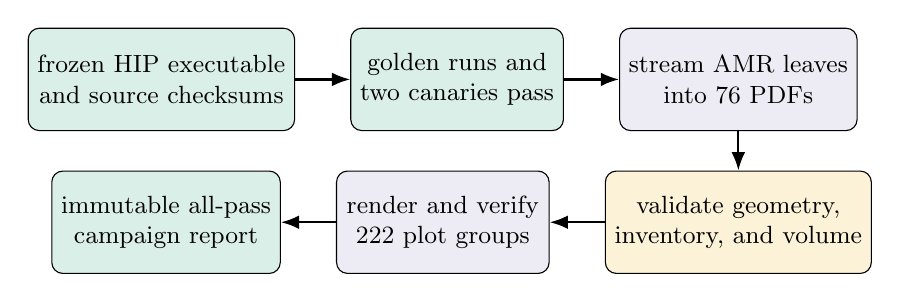
\begin{tikzpicture}[>=Latex,
  node distance=5mm and 7mm,
  box/.style={draw,rounded corners,minimum width=27mm,minimum height=13mm,
              align=center,font=\small},
  gate/.style={box,fill=trusted!16},
  work/.style={box,fill=gpu!13},
  check/.style={box,fill=caution!16}]
\node[gate] (freeze) {frozen HIP executable\\and source checksums};
\node[gate,right=of freeze] (gates) {golden runs and\\two canaries pass};
\node[work,right=of gates] (reduce) {stream AMR leaves\\into 76 PDFs};
\node[check,below=of reduce] (manifest) {validate geometry,\\inventory, and volume};
\node[work,left=of manifest] (plots) {render and verify\\222 plot groups};
\node[gate,left=of plots] (campaign) {immutable all-pass\\campaign report};
\draw[->,thick] (freeze)--(gates);
\draw[->,thick] (gates)--(reduce);
\draw[->,thick] (reduce)--(manifest);
\draw[->,thick] (manifest)--(plots);
\draw[->,thick] (plots)--(campaign);
\end{tikzpicture}
\caption{The publication chain. A production result becomes acceptable only
after every gate to its left has passed. The diagram is a schematic, not
evidence.}
\end{figure}

The PDFs themselves are additive reductions. For product \(p\), each native
AMR leaf cell \(c\) contributes a weighted cell volume to one bin:
\[
H_p(b)=\sum_c \Delta V_c\,w_p(c)\,
  \mathbf{1}\!\left[B_p(\boldsymbol{q}_c)=b\right].
\]
That structure makes a streaming MPI+Kokkos reducer possible. Each rank reads
its assigned shard, bins bounded chunks on the GPU, and participates in global
reductions. No global dense simulation cube is assembled.

That only works if the input cells really are the intended snapshot. The
production validator therefore checks more than histogram sums. It maps
geometry back to logical AMR keys, rejects duplicate leaves and
ancestor--descendant overlap, requires the exact contiguous shard inventory,
and checks that leaf volumes close to the domain volume. Product payloads are
published atomically through temporary \codeword{.partial} files, and the
snapshot manifest is written last.

\section{What was actually done}

\subsection{A release identity was frozen before production}

The production executable and source set were frozen into a release identity.
The identity records the HIP executable, source bundle, reducer source, and
source-tree revision. Their identifiers begin with
\codeword{ea53c3cf0f2e}, \codeword{0cbb0da68c25},
\codeword{ffce7ab54296}, and \codeword{db953863b6c0}, respectively; the
complete hashes are in the artifact map below.

Production workers did not merely point at an executable path. Before each
task, they verified the immutable release identity and five immutable passing
reports: three golden runs, a 256-node canary, and a no-control canary. This
made ``the tested binary'' and ``the production binary'' the same verifiable
object.

\begin{table}[ht]
\centering
\small
\begin{tabular}{lrrrrl}
\toprule
Gate & Job & Nodes & Shards & Reducer time & Validator \\
\midrule
golden original & 4767325 & 128 & 1024 & 5.97 s & 31 pass, 0 fail \\
golden science  & 4767326 & 128 & 1024 & 6.21 s & 22 pass, 0 fail \\
golden all      & 4767327 & 128 & 1024 & 7.11 s & 42 pass, 0 fail \\
256-node canary & 4767328 & 256 & 2048 & 4.39 s & 41 pass, 0 fail \\
no-control canary & 4767329 & 64 & 512 & 4.20 s & 26 pass, 0 fail \\
\bottomrule
\end{tabular}
\caption{The completed Frontier release ladder. Every run also passed
geometry-to-logical-key validation and its predeclared performance budget.
Source: immutable golden and canary pass reports recorded by the release
identity and final traceability record.}
\end{table}

\subsection{Calculation, plotting, and campaign acceptance were separate gates}

For each snapshot, the reducer first verified the input headers and exact
shard inventory. During reduction it rejected malformed records, invalid
hydrodynamic states, duplicate AMR leaves, and logical-key overlap. It then
required domain-volume closure and wrote 76 products. The completed snapshot
manifest was the last publication step.

The plot driver accepted only a completed, validated snapshot manifest. It
rendered each product's profiles and pairwise heatmaps, wrote per-product
metadata, generated an index, and verified the completed plot root. The
campaign validator then independently walked the full expected inventory. It
checked the calculation identities, source sequences and times, shard counts,
geometry-validation flags, product files and finite sums, plot metadata,
expected PNG counts, indexes, provenance hashes, audited source views, missing
outputs, unexpected outputs, and partial artifacts.

\section{The evidence that matters}

The final trust anchor is the immutable report
\codeword{production-campaign.8fd47b0c...49388a.json}. It was generated on
June 6, 2026 at 02:32 UTC and has status \pass. Its summary is:

\begin{table}[ht]
\centering
\begin{tabular}{lr}
\toprule
Measure & Verified result \\
\midrule
Expected and completed calculations & 161 / 161 \\
Expected and completed plot sets & 161 / 161 \\
Products per snapshot & 76 \\
Plot groups per snapshot & 222 \\
Total PNG plot groups & 35,742 \\
Total native cells processed & 11,099,956,051,968 \\
Source payload bytes read & 355,202,319,844,512 \\
Reducer elapsed-time range & 2.79--71.11 s \\
Reported errors & 0 \\
Missing calculations / plot sets & 0 / 0 \\
\bottomrule
\end{tabular}
\caption{Campaign-level results read directly from the immutable final report.}
\end{table}

\begin{table}[ht]
\centering
\begin{tabular}{lr}
\toprule
Simulation & Validated snapshots \\
\midrule
\codeword{res\_4pc} & 29 \\
\codeword{res\_4pc\_highmdot} & 28 \\
\codeword{res\_8pc} & 49 \\
\codeword{res\_8pc\_lowmdot} & 25 \\
\codeword{res\_8pc\_highmdot} & 30 \\
\midrule
Total & 161 \\
\bottomrule
\end{tabular}
\caption{The five-simulation inventory accepted by the final campaign
validator.}
\end{table}

The report is stronger than a count of Slurm completions. Its campaign
validator SHA-256 is itself recorded
(\codeword{30b4a8137497bb19...d0cf}), as are the release identity, golden and
canary reports, plot driver, plotter, snapshot inventory, and the corrected
source manifest described below. The report and its SHA-256 sidecar are
read-only under the release directory.

\section{The failure that mattered}

The most useful event in the campaign was a failure. The original source
directory for snapshot
\codeword{res\_8pc\_highmdot}/\codeword{phase1}/\codeword{00000} contained
250 shard directories. They did not all belong to one snapshot:
\begin{itemize}
  \item \codeword{node\_00000000} through \codeword{node\_00000199} were the
        contiguous May 12 snapshot;
  \item \codeword{node\_00000200} through \codeword{node\_00000249} were stale
        May 7 files.
\end{itemize}

The tempting approach would have been to trust the directory count and process
all 250 shards. That run was attempted, and the reducer rejected it because
global AMR validation found duplicate logical leaf keys. No manifest was
published for the bad input.

The corrected run used an explicit, audited source view containing exactly the
200 current shards. Corrected job 4769652 then validated 25,192 unique AMR
leaves, closed the domain volume to \(64{,}000{,}000.000000089\), processed
6,603,931,648 cells, and completed in 4.049 seconds. The final report preserves
the reason for the override, the included and excluded node ranges, both
mtime ranges, and a SHA-256 over the source-view entry metadata.

\bottomline This incident is evidence that the validation was active rather
than ceremonial. A superficially complete shard directory failed closed; the
campaign accepted only the audited full snapshot.

\section{What worked, and what did not}

What worked:
\begin{itemize}
  \item the frozen HIP release passed the full 1024-shard golden sequence,
        2048-shard scaling canary, and no-control validation before production;
  \item all 161 intended snapshots produced validated 76-product manifests;
  \item all 161 snapshots produced verified 222-group plot roots and indexes;
  \item the final campaign validator found no errors or missing calculations
        or plots;
  \item the stale-shard input was rejected before publication and replaced by
        a traceable audited source view.
\end{itemize}

Several operational attempts did not work. Frontier submission limits required
staged submission. Thirty-two early retries failed immediately because an
external helper passed an empty \codeword{MANIFEST\_PATH}; they created no
accepted source or output artifact. One source-view precheck failed because
its \codeword{find} invocation did not follow directory symlinks; the corrected
helper did, without changing the reducer or release checks. These attempts
remain visible in the logs, but none were accepted by the final report.

The important engineering result is not that every attempt succeeded. It is
that failed attempts could not satisfy the publication contract.

\section{What the result means}

The completed campaign strongly supports this claim:

\begin{quote}
For every snapshot in the declared 161-snapshot production inventory, the
frozen reducer processed an exact, globally validated AMR leaf set, published
the expected 76 reconstructed PDF products, and the frozen plotting path
published the expected 222 verified plot groups. The immutable campaign
validator found no missing or inconsistent accepted result.
\end{quote}

That is the claim this work was designed to establish. It means the
reconstructed products and plots are ready to be used for scientific analysis,
with the immutable campaign report as the root of trust.

It does \emph{not} prove every possible scientific interpretation of those
PDFs. In particular:
\begin{itemize}
  \item the same-state bad-line/fixed-line AthenaK A/B run remains the cleanest
        causal proof of the original archive corruption;
  \item the independent oracle covers all 14 original products but only 20 of
        62 science products;
  \item the campaign validates this declared reconstruction model and product
        catalog; it does not validate unrelated magnetic, particle, history,
        or cooling diagnostics;
  \item numerical agreement with an online double-precision implementation is
        not a claim of bitwise identity.
\end{itemize}

Those are scientific-validation limits, not missing production outputs.

\section{How to use the result}

Use the immutable campaign report as the first acceptance check, then follow
its recorded provenance to the snapshot manifest and per-product plot
metadata. Do not infer acceptance from a Slurm exit code or from the presence
of a plot directory alone.

The primary artifacts are:

\begin{description}
  \item[Immutable campaign report]\hfill\\
  \evidencepath{/lustre/orion/ast207/proj-shared/gotham/analysis/products/pdf_rebuild/release/}\\
  \evidencepath{production-campaign.8fd47b0c5cc8b405779e37fc865685aa255088bb6aeaa00e389de953ee49388a.json}
  \item[Frozen release identity]\hfill\\
  \evidencepath{/lustre/orion/ast207/proj-shared/gotham/analysis/products/pdf_rebuild/release/}\\
  \evidencepath{frontier-release-identity.7a517368fe384bc3e793dca9bea96ff0042a5a6995815be1ceb25ab5abd9cf4f.json}
  \item[Validated calculation roots]\hfill\\
  \evidencepath{/lustre/orion/ast207/proj-shared/gotham/analysis/products/pdf_rebuild/production}
  \item[Verified plot roots]\hfill\\
  \evidencepath{/lustre/orion/ast207/proj-shared/gotham/analysis/products/pdf_rebuild_plots/production}
  \item[Final traceability record]\hfill\\
  \evidencepath{/ccs/home/dfielding/athenak-gotham-pdf-rebuild/docs/explanatory_writeups/FINAL_TRACEABILITY.md}
\end{description}

\section{Subsequent visualization replacement}

The immutable campaign report records the original 35,742-plot release-gated
campaign. On June 6, 2026, that visible plot tree was replaced by a
user-approved scientific suite: 165 descriptive PNG views for each of the 161
snapshots, or 26,565 PNGs total, plus 1,155 H.264/YUV420p MP4 movies. PNG and
movie filenames no longer use opaque \texttt{outputXX} labels, and uniform
branches are separate movie series.

This replacement did not alter the validated reducer outputs, frozen release
identity, or immutable campaign report. The current visualization audits are:

\begin{description}
  \item[Current plot campaign manifest]\hfill\\
  \evidencepath{/lustre/orion/ast207/proj-shared/gotham/analysis/products/pdf_rebuild_plots/production/}\\
  \evidencepath{plot_campaign_manifest.json}
  \item[Current movie campaign manifest]\hfill\\
  \evidencepath{/lustre/orion/ast207/proj-shared/gotham/analysis/products/pdf_rebuild_plots/production/movies/}\\
  \evidencepath{movie_manifest.json}
\end{description}

\section{Bottom line}

The full PDF calculation and plotting campaign reached the intended terminal
state: 161 validated snapshot calculations, 12,236 PDF products, and 35,742
verified PNG plot groups under one frozen release identity. The strongest
reason to trust the result is not the final count. It is that the system
rejected a real mixed-snapshot shard directory, required an audited correction,
and recorded that exception in the same immutable report that accepts the
other 160 snapshots.

The current visible visualization suite is the later descriptive replacement:
26,565 PNGs and 1,155 QuickTime-compatible movies.

The remaining uncertainty is narrower: production completeness is established,
but some scientific claims still need broader external-oracle coverage and the
clean same-state AthenaK A/B causal test.

\end{document}
